\chapter{Introduction}

\section{Programming Languages Are Useful in Enforcing Security Policies}

With the development of digital society, people are increasingly
concerned about the confidentiality of their personal data and
the integrity of their online assets. Increasingly relying on
computing devices and the Internet in their daily life, people fear that
sensitive personal information, such as social security numbers,
medical records, bank account balances... may be revealed to malicious
third parties. People also worry that their digital photo albums,
signatures on online legal documents, spreadsheets in cloud storage...
may be tampered and manipulated by potential attackers.

Indeed, the fears are justified by recent news events.
In 2018, the Cambridge Analytica scandal hit the world headlines,
where the data collected from 87 million social media users was misused
without their consent
~\parencite{cadwalladr2018facebook,kitchgaessner2017cambridge,gonzalez2019global,hinds2020wouldn}.
In the healthcare sector, from 2005 to 2019, 249.09 million individuals
were affected by data breaches that caused exposure of sensitive medical
data~\parencite{seh2020healthcare}. In respect of data integrity, researchers
have found ways to tamper the analytics APIs~\parencite{pfeffer2018tampering} and
the metadata (such as the numbers of likes, follows, and views)~\parencite{paquet2017can}
of major social media platforms. To deal with the security and privacy
challenges of the increasingly digitalized world, the European Union introduced
the General Data Protection Regulation (GDPR) to reform and regulate
the collection and processing of personal data. However, studies show
that business entities experience challenges in complying with GDPR
or auditing for compliance~\parencite{smirnova2024understanding},
particularly small-to-medium enterprises~\parencite{sirur2018we,freitas2018gdpr,harting2021impacts}.

\begin{figure}[tbp]
  \small
  \begin{align*}
    \langle RECORD \rangle ::= & {\color{green} \textbf{\{FirstName=}} \langle ID \rangle {\color{green} \textbf{;}} \\
                               & \enspace {\color{green} \textbf{LastName=}} \langle ID \rangle {\color{green} \textbf{;}} \\
                               & \enspace {\color{green} \textbf{SSN=}} \langle SSN \rangle {\color{green} \textbf{\}}} \\
    \langle ID \rangle     ::= & w , w \in \{ {\color{green} \textbf{A}}, ... {\color{green} \textbf{Z}}, {\color{green} \textbf{a}}, ... {\color{green} \textbf{z}} \}^{+} \\
    \langle SSN \rangle    ::= & \langle D \rangle \langle D \rangle \langle D \rangle {\color{green} \textbf{-}}
                                 \langle D \rangle \langle D \rangle {\color{green} \textbf{-}}
                                 \langle D \rangle \langle D \rangle \langle D \rangle \langle D \rangle \\
    \langle D \rangle      ::= & d , d \in \{ {\color{red} \textbf{0}}, ... {\color{red} \textbf{9}} \}
  \end{align*}
  \caption{The user input grammar for a hypothetical application}
  \label{fig:grammar}
\end{figure}

From a technical perspective, ensuring the security and privacy of
personal data typically involves tracking and checking
the flow of information.
Modern software applications often accept user input where
selected fields are sensitive, whose confidentiality is required
during both parsing and processing. To rule out information leaks,
neither the sensitive fields, nor any data that depends on those fields,
is allowed to be revealed to a low-privilege observer.
Consider a web application that receives three fields from its user:
\Circled{1} first name \Circled{2} last name \Circled{3}
social security number, the grammar of which
is defined in Figure~\ref{fig:grammar}, where terminals are divided into
low-security and high-security.
The digits $d$ for social security number, being confidential to users of
the web application, are of high-security, so they are marked {\color{red}
  red}, while other terminals, such as the keys of the record and the
strings $w$ for first name / last name, being safe to disclose, are
all of low-security, marked in {\color{green} green}.

Consider the following user input:

\begin{lstlisting}[numbers=none,xleftmargin=0.1\textwidth]
{FirstName=Mad;LastName=Hatter;SSN=012-34-5678}
\end{lstlisting}

It is tedious for the developer of this imaginary web application
to track the security level of data and check for information leaks.
Software developers tend to focus more on functionality
in order to meet the tight software release schedule and budget,
thus software security usually only comes as an afterthought
~\parencite{assal2018security,sharma2017aspects,steward2012software}.
Retrofitting security-related code often requires extensive modification to
an existing code-base and it relies on the programmers' skills
and experience to decide when and where such code should be placed.
Furthermore, such modification is error-prone: one single missing
check could undermine the security of the entire application.

Alternatively, the author of the web application could implement
a parser for the grammar in Figure~\ref{fig:grammar} in
a \textit{programming language} that enforces information-flow security.
Each terminal in the grammar would be labeled with a security level and
the programming language, instead of some ad-hoc checks implemented by
the programmer of the web application, would guarantee that
the high-security information is only present in those parts of
the output parse tree that are marked as high-security.
For example, according to the grammar in Figure~\ref{fig:grammar},
the example user input string is parsed into the parse tree in
Figure~\ref{fig:parsetree}, where the terminal nodes that represent digits of
the social security number are of {\color{red} high-security},
while the terminals that compose the rest of the input string are of
{\color{green} low-security}.  The confidentiality of SSN is guaranteed
during data processing since the programming language enforces
noninterference. When the web application interacts with the outside
world, such as making a foreign function interface (FFI) call
or storing into a database, the conceptual language should encrypt
whatever values labeled as high security before they are passed into a
foreign routine. The programming language-based approach of
information-flow security~\parencite{sabelfeld2003language}
alleviates the security burden of software development,
because it forms an abstraction over the flows of information and
decouples security from the functionality of a software application.

\begin{figure*}[tbp]
  \small
  \center
\begin{tikzpicture}[scale=0.8]
\tikzset{level distance=40pt}
\Tree [
  .{ $\langle RECORD \rangle$ }
  {\color{green} \textbf{\{FirstName=}}
  [ .{ $\langle ID \rangle$ } {\color{green} \textbf{Mad}} ]
  {\color{green} \textbf{;LastName=}}
  [ .{ $\langle ID \rangle$ } {\color{green} \textbf{Hatter}} ]
  {\color{green} \textbf{;SSN=}}
                       [ .{ $\langle SSN \rangle$ }
                         [ .{ $\langle D \rangle$ } {\color{red} \textbf{0}} ]
                         [ .{ $\langle D \rangle$ } {\color{red} \textbf{1}} ]
                         [ .{ $\langle D \rangle$ } {\color{red} \textbf{2}} ]
                         {\color{green} \textbf{-}}
                                [ .{ $\langle D \rangle$ } {\color{red} \textbf{3}} ]
                                [ .{ $\langle D \rangle$ } {\color{red} \textbf{4}} ]
                                {\color{green} \textbf{-}}
                                       [ .{ $\langle D \rangle$ } {\color{red} \textbf{5}} ]
                                       [ .{ $\langle D \rangle$ } {\color{red} \textbf{6}} ]
                                       [ .{ $\langle D \rangle$ } {\color{red} \textbf{7}} ]
                                       [ .{ $\langle D \rangle$ } {\color{red} \textbf{8}} ] ]
                       {\color{green} \textbf{\}}}
]
\end{tikzpicture}
\caption{The parse tree generated from the example user input.
  All terminals are represented as labeled values:
  the {\color{red} red} ones, such as the digits of SSN,
  are of high-security, while the {\color{green} green} ones, such as the keys
  of the record and first name / last name, are of low-security.}
\label{fig:parsetree}
\end{figure*}

\section{Mechanisms of Programming Language-Based
  Information-Flow Control: Static, Dynamic, and Gradual}

Information-flow control (IFC) ensures that information transfers
within a program adhere to a security policy, for example, by
preventing high-security data from flowing to a low-security
channel.
Traditionally, a programming language can enforce IFC either statically
using a security type system~\parencite{volpano1996sound,Myers:1997aa,myers1999jflow},
or dynamically using runtime monitoring
~\parencite{Askarov:2009vq,austin2009efficient,Devriese:2010up,stefan2011flexible,Austin:2017uh},
or with a combination of the two
~\parencite{le2005monitoring,le2007automaton,Chandra:2007we,Shroff:2007tg}.
The two approaches have complementary strengths and weaknesses;
the dynamic approach requires less effort from the programmer
while the static approach provides stronger guarantees and
less runtime overhead. Recently, there has been increasing interest in
building gradual security-typed languages: taking inspiration from
gradual typing~\parencite{Siek:2006bh,Siek:2007qy,Tobin-Hochstadt:2006fk, Matthews:2007zr},
researchers have explored how to give programmers seamless control over
which parts of the program are secured statically versus dynamically.

\textbf{Static IFC in programming languages}
The interest in enforcing confidentiality and regulating the flow of
information in a computer program arises with its defense applications
in the 1970s \autocite{bell1976secure}.
\textcite{denning1976lattice}
builds a information flow model using a lattice of security labels and
\textcite{denning1977certification} discuss the certification technique
in further detail, with a proof that a certified program will not give
away confidential input from non-confidential output.
\textcite{volpano1996sound} propose a typed-based approach to enforcing
information flow, by defining a type system for an imperative
programming language and proving its security with a type soundness
proof. This idea is further developed by
\textcite{zdancewic2002programming}.  Such a protection scales well since
type checking is \textit{compositional}
\parencite{sabelfeld2003language}. There are projects that apply similar
techniques but to other languages
such as bytecode intermediate languages
\autocite{barthe2005non}, object-oriented languages
\autocite{amtoft2006logic}, and reactive programming languages
\autocite{bohannon2009reactive}. Although the aforementioned languages are
mostly theoretical, efforts have also been made to integrate information
flow control into widely-used existing languages such as \textit{Jif}
for Java \autocite{myers1999jflow} and \textit{Flow Caml} for OCaml
\autocite{pottier2002information, simonet2003flow}.

\textbf{Dynamic IFC in programming languages}
\textcite{li2006encoding,LI20101974} add flow control to Haskell by utilizing
existing language features, specifically arrow and typeclass,
to implement checks.
\textcite{stefan2011flexible,stefan2012flexible,STEFAN:2017ta}
design a Haskell library called \textit{LIO};
inspired by IFC operating systems
~\parencite{efstathopoulos2005labels,zeldovich2011making,krohn2007information,vandebogart2007labels},
\textit{LIO} takes a coarse-grained, floating-label approach that
employs a labeled IO monad to keep track of the current privilege level,
which restricts both the observability and the security effect.
\textcite{austin2009efficient} consider IFC for Javascript and
propose a purely dynamic approach called no-sensitive-upgrade
checking to handle implicit flows through the heap.

\textbf{\purpletext{Gradual IFC in programming languages}}

\section{The Tension Between Noninterference and the Gradual Guarantee}

\section{Thesis Statement}

\section{Contributions and Outline}
